\subsection{Overview}

We introduce a framework that evaluates large language models not only as direct task solvers but as assistants that help another agent do the work. We study two usage modes. In the \emph{automation} mode, as in most existing benchmarks, a focal model completes a professional task end-to-end. In the \emph{augmentation} mode, a fixed lower-capability worker
model completes the task with help from an assistant model: the worker requests assistance, the assistant model replies with an assistance text - a plan, checklists, constraints, and self-review steps - and the worker uses that support to produce the final deliverable. The assistant model never writes the deliverable itself, so what varies across augmentation trials is the quality of its guidance, not whether it simply did the work. We use GPT-3.5-Turbo as the
worker for two reasons: it approximates worker performance on our pilot tasks, and it represents the cheaper, lower-capability models that are often assigned the execution role in multi-agent settings. Figure~\ref{fig:methodology-pipeline} summarizes the full workflow.

Every output is evaluated in both usage modes through blind pairwise comparisons by a panel of four LLM judges using task-specific and general rubrics. Each judge is barred from scoring outputs produced by its own model family (leave-one-family-out masking) to limit self-preference, and we replicate the full pipeline across ten independent runs. The result is a cross-mode, cross-task rank matrix over ten models: Claude-Opus-4.8, Claude-Sonnet-4.6, Gemini-3.1-Pro, DeepSeek-V3.1, GPT-5-Mini, GPT-OSS-120B, GPT-O4-Mini, GPT-4.1, GPT-O3-Mini, and GPT-3.5-Turbo. For each model, we can ask not only whether it ranks higher as a direct solver or as an assistant, but also whether that ordering holds across tasks. The framework therefore produces a profile for each model rather than a single score. A model may complete structured execution tasks well on its own yet be a weaker assistant on open-ended, human-facing tasks; another may rank lower as a direct solver but produce assistance text that clearly improve counseling, tutoring, or planning outputs. Capturing this split is our core methodological
contribution.

\begin{figure}[htbp]
\centering
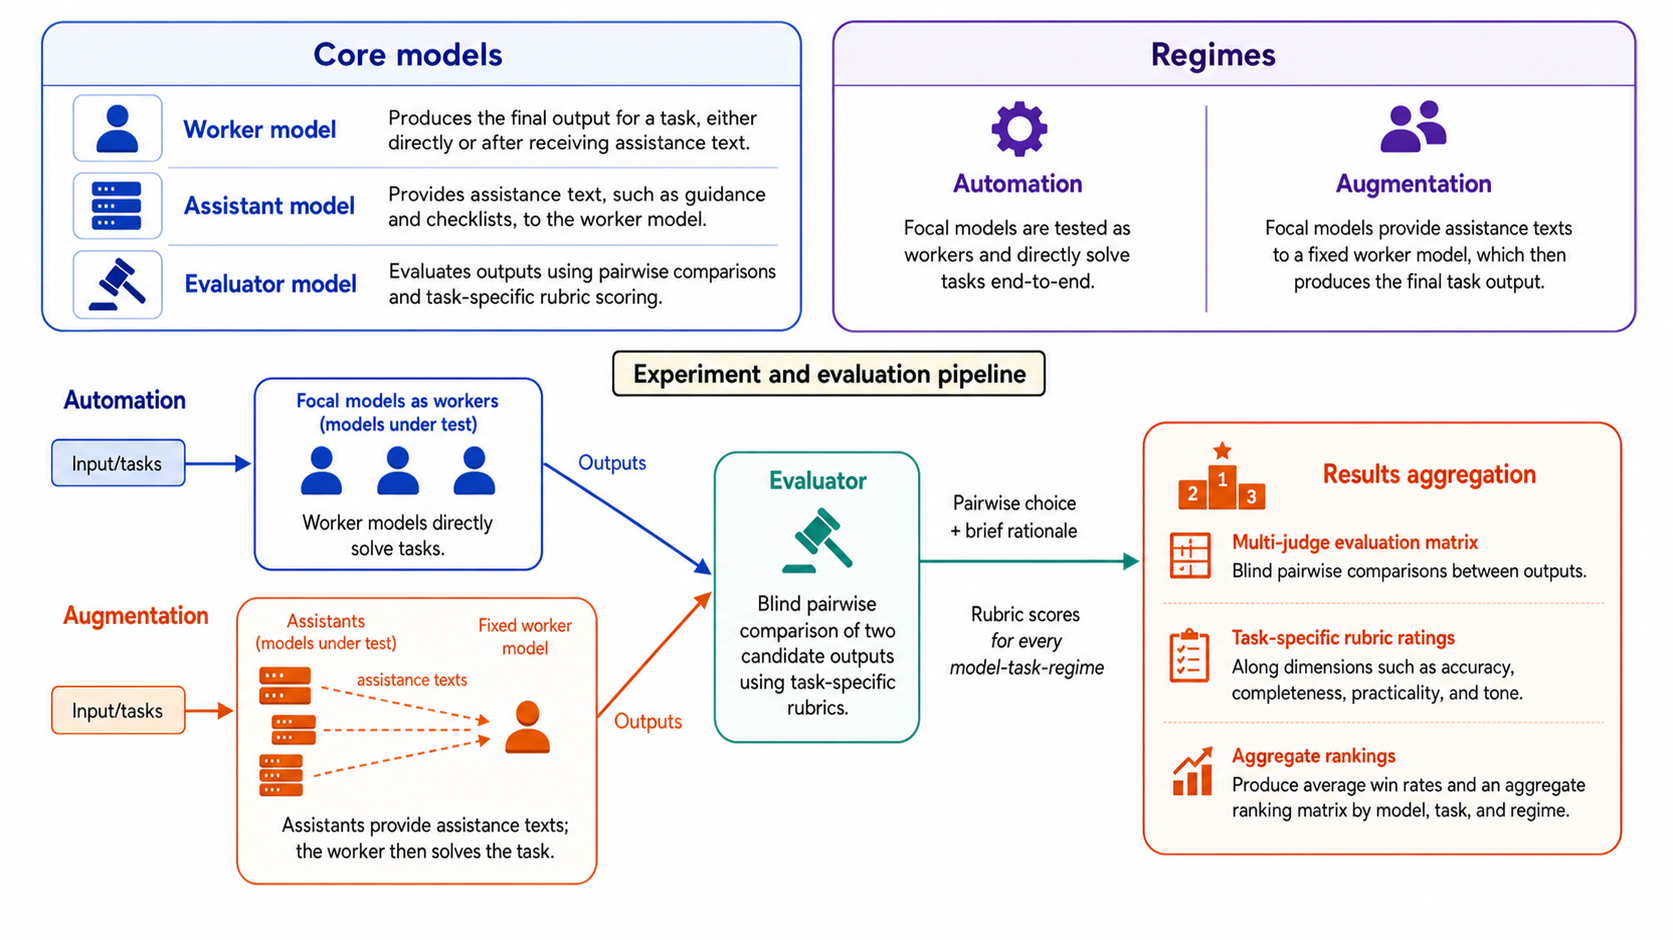
\includegraphics[width=\linewidth]{figures/methodology-final.png}
\caption{\textbf{Methodology pipeline.} The framework evaluates models in two usage modes: automation, where focal models directly solve tasks, and augmentation, where focal models provide an assistance text to a fixed worker model. Outputs are evaluated through rubric-guided pairwise comparisons and aggregated into model rankings by task and usage mode.}
\label{fig:methodology-pipeline}
\end{figure}


\subsection{Task Selection and Prompt Design}

We construct a benchmark of seven tasks representing activities commonly encountered in everyday and professional settings and associated with economically meaningful forms of work: counseling, market analysis, meal planning, operations research, tax preparation, travel planning, and tutoring. Tasks were chosen to vary in structure, domain knowledge, risk, and the degree to which human-facing judgment matters. Each task specifies an observable deliverable with concrete requirements, allowing evaluation to assess whether outputs satisfy stated constraints objectively rather than relying on subjective impressions of quality. Figure~\ref{fig:tasks} presents the full task set. The assistant model set and judge panel are reported in the supplementary document.

To make evaluation reliable, each task prompt is paired with a micro-rubric. The prompt specifies the required deliverable and the components that must be present. The rubric mirrors those components and scores each dimension on a 1--10 scale. Each task includes task-specific dimensions, such as dietary safety for meal planning or mathematical correctness for tutoring, as well as general dimensions such as instruction following, accuracy, practical usefulness, organization, and tone. We evaluate models pairwise to enable contrastive grading (which we found worked better), where the judge can compare models to determine winners rather than grade inherently subjective outputs. However, we also develop the task-specific rubrics to help ground the judge's decision, and also as a way for humans to reason about why certain outputs were judged better than others. 


\begin{figure}[htbp]
\centering
%
\includegraphics[width=\linewidth]{tasks.png}
\renewcommand{\arraystretch}{1.15}
\setlength{\tabcolsep}{6pt}
\small

\definecolor{planyellow}{RGB}{255,247,222}
\definecolor{profgreen}{RGB}{231,243,231}
\definecolor{humanpurple}{RGB}{237,236,250}
\definecolor{headnavy}{RGB}{16,42,94}

\begin{tabularx}{\linewidth}{
    >{\raggedright\arraybackslash\hsize=0.85\hsize}X
    >{\raggedright\arraybackslash\hsize=1.05\hsize}X
    >{\raggedright\arraybackslash\hsize=1.00\hsize}X
    >{\raggedright\arraybackslash\hsize=1.10\hsize}X}
\toprule
\rowcolor{headnavy}
\textcolor{white}{\textbf{Task}} &
\textcolor{white}{\textbf{Source}} &
\textcolor{white}{\textbf{Task type}} &
\textcolor{white}{\textbf{Deliverable}} \\
\midrule
\rowcolor{planyellow}
Menu Planning & GDPval & Structured planning & Seven-day constrained meal plan \\
\rowcolor{planyellow}
Travel Planning & GDPval & Structured planning & Tokyo itinerary under fixed budget \\
\rowcolor{profgreen}
Market Trends Analysis & GDPval & Professional / analytical & Client brief on natural gas trends \\
\rowcolor{profgreen}
Operations Research Analysis & Anthropic Economic Index & Professional / analytical & Executive logistics optimization memo \\
\rowcolor{profgreen}
Tax Preparation & Designed task & Professional / analytical & Tax discrepancy review and correction guidance \\
\rowcolor{humanpurple}
Counseling & Anthropic Economic Index & Human-facing interactive & Supportive counseling-style response \\
\rowcolor{humanpurple}
Tutoring Session Planning & Anthropic Economic Index & Human-facing interactive & Grade 3 lesson segment \\
\bottomrule
\end{tabularx}
\caption{\textbf{Tasks included in the benchmark.}
    The figure reports each task's source, broad task type, and required deliverable. Colors distinguish structured-planning tasks (yellow), professional or analytical tasks (green), and human-facing interactive tasks (purple). Tasks were drawn from GDPval and the Anthropic Economic Index, except for tax preparation, which was designed by the authors to provide a rule-based professional task with verifiable discrepancies. Full task prompts and evaluation rubrics are provided in the supplementary document.}
\label{fig:tasks}
\end{figure}


This alignment between prompt and rubric is central to the framework. We do not ask evaluators to make an undifferentiated and subjective judgment of quality. Instead, they judge whether the response satisfies observable dimensions of the task that are quantifiable and comparatively objective to assess. For example, the travel-planning rubric separately measures cost realism, itinerary quality, hotel and transportation practicality, and handling of uncertainty. Meanwhile, the tax-preparation rubric separately measures rule accuracy, discrepancy detection, calculation quality, form guidance, dependent analysis, and client-facing clarity. Figure~\ref{fig:prompt-rubric-design} summarizes the alignment between task prompts, task-specific micro-rubrics, general evaluation dimensions, and the augmentation assistance text constraint.

\begin{figure}[htbp]
\centering
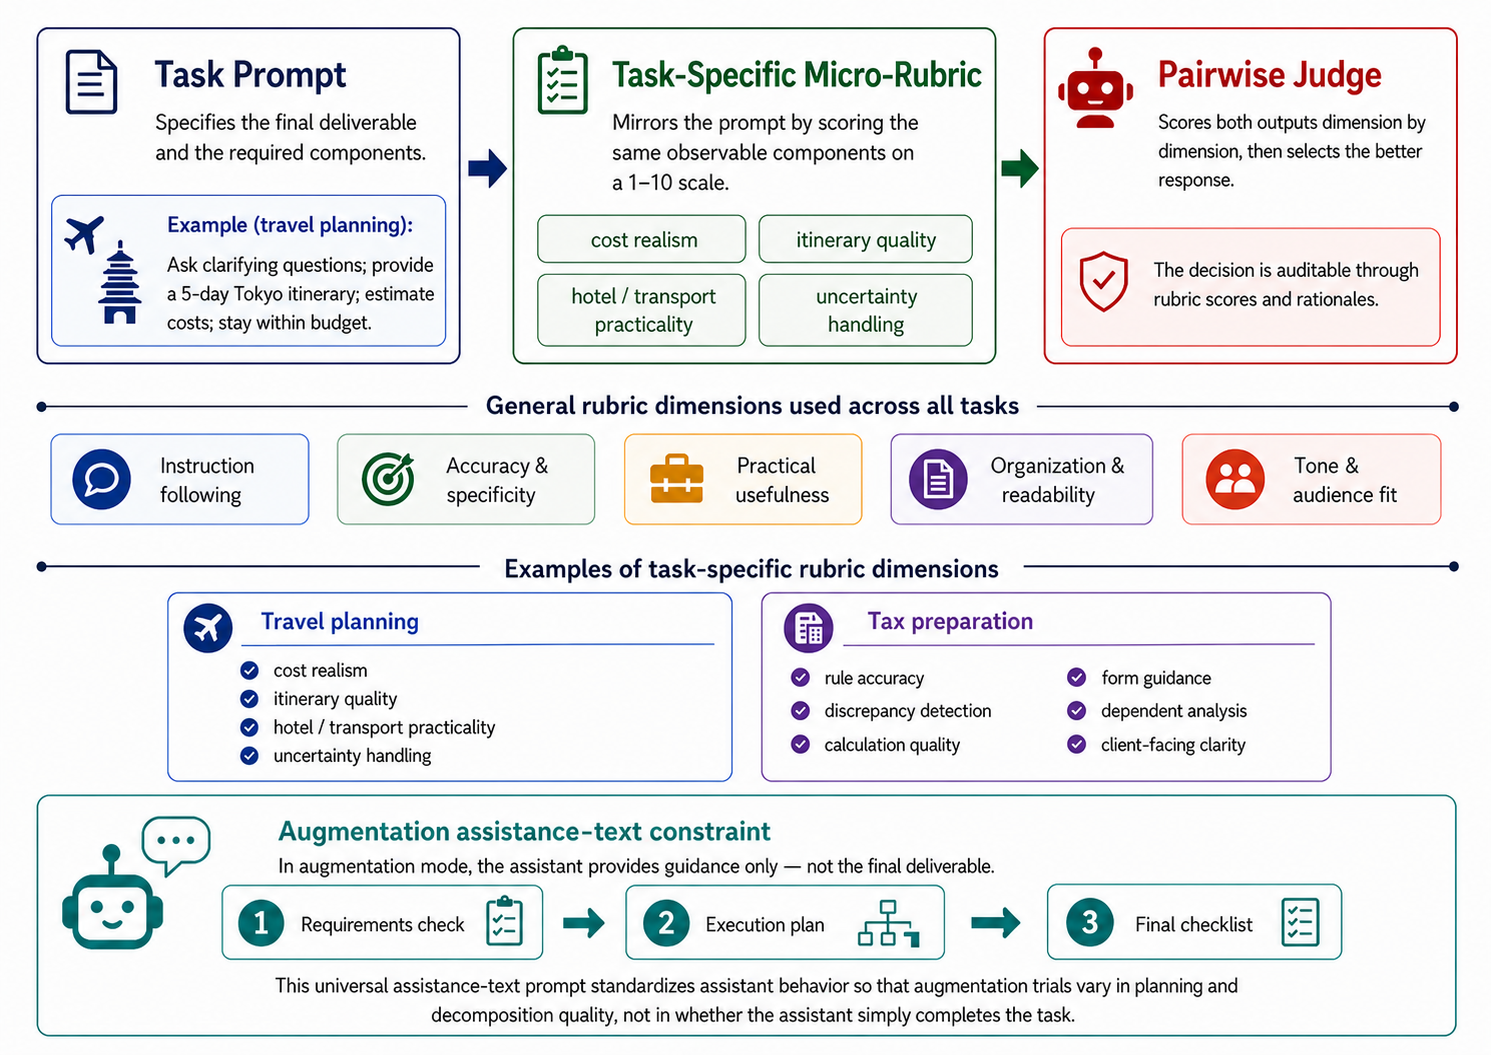
\includegraphics[width=\linewidth]{figures/evals-final.png}
\caption{\textbf{Prompt and rubric design.} Each task prompt specifies observable deliverable requirements, which are mirrored by task-specific micro-rubrics. General rubric dimensions are held constant across tasks, while task-specific dimensions vary by domain. In augmentation mode, the assistance text creation prompt constrains assistant models to provide process guidance rather than the final deliverable.}
\label{fig:prompt-rubric-design}
\end{figure}


Figure~\ref{fig:prompt-rubric-example} illustrates the prompt and rubrics for travel planning. Full prompts, assistance texts, and rubrics for all tasks appear in the supplementary document. In augmentation mode, each assistant model receives a universal assistance text creation prompt that instructs it to produce a process-oriented plan for the worker, rather than completing the task itself. The prompt specifies a three-phase structure: a requirements check, an execution plan, and a final checklist. It additionally constrains the assistant to provide guidance only, explicitly prohibiting production of the final deliverable. This design ensures that what varies across augmentation trials is the quality of the assistant's planning and decomposition, not whether the assistant simply solved the task on the worker's behalf. 


\begin{figure}[htbp]
\centering
\footnotesize

\definecolor{taskblue}{RGB}{220,235,252}
\definecolor{taskblueframe}{RGB}{16,42,94}
\definecolor{rubricmint}{RGB}{225,245,225}
\definecolor{rubricmintframe}{RGB}{16,42,94}
\definecolor{assistpeach}{RGB}{255,242,218}
\definecolor{assistpeachframe}{RGB}{16,42,94}


\scalebox{0.95}{%
\begin{minipage}{\linewidth}
\begin{tcolorbox}[taskprompt, enhanced, colback=taskblue, colframe=taskblueframe, colbacktitle=taskblueframe, coltitle=white, title=Task Prompt --- Travel Planning]
Create a 5-day Tokyo itinerary for one traveler next month with a total budget of \$2,500 USD, excluding passport costs. The traveler is departing from San Francisco. Clearly state assumptions and give clarifying questions before the provisional plan. Use realistic estimates, label them as estimates, and keep the plan budget-aware.
\end{tcolorbox}

\vspace{0.4em}

\begin{tcolorbox}[rubricbox, enhanced, colback=rubricmint, colframe=rubricmintframe, colbacktitle=rubricmintframe, coltitle=white, title=Evaluation Rubric --- Travel Planning]
Score each dimension from 1 (lowest) to 10 (highest):
\begin{enumerate}
  \setlength{\itemsep}{0pt}
  \item Completeness: covers questions, costs, hotels, transport, customs/regulations, itinerary, and budget confirmation.
  \item Cost realism and arithmetic: flights, lodging, transport, food/activities, and total are plausible and correctly summed. Penalize outputs that exceed the budget.
  \item Hotel and transport practicality: viable hotel options, airport/transit guidance, rail/pass advice.
  \item Itinerary quality: 5 days with morning/afternoon/evening plans that are geographically sensible and well-optimized for distance and fatigue.
  \item Travel-agent professionalism: clear, customer-focused, with appropriate caveats around estimates.
  \item Handling uncertainty: asks clarifying questions for missing information while still providing a useful provisional plan.
\end{enumerate}
\end{tcolorbox}
\end{minipage}}

\vspace{0.4em}

\scalebox{0.95}{%
\begin{minipage}{\linewidth}
\begin{tcolorbox}[taskprompt, enhanced, fonttitle=\bfseries, colback=assistpeach, colframe=assistpeachframe, colbacktitle=assistpeachframe, coltitle=white, title=Assistance Text Creation Prompt --- Universal (Abridged)]
Produce a 200--250 word, process-focused assistance text without writing the final deliverable.

Organize the assistance text into three phases:
\begin{enumerate}
    \setlength{\itemsep}{1pt}
    \item \textbf{Requirements Check:} identify the deliverable, audience, tone, constraints, and required components.
    \item \textbf{Plan and Structure:} recommend a general response structure and explain how to balance completeness, clarity, and tone.
    \item \textbf{Self-Review and Finalize:} provide a concise checklist for reviewing the response before submission.
\end{enumerate}

Do not solve the task, provide task-specific content or examples, or write sentences that could be copied into the final answer. Keep the guidance process-focused.

\medskip
\textit{Abridged for presentation. The full verbatim experimental prompt is provided in the supplementary document.}
\end{tcolorbox}
\end{minipage}}

\caption{\textbf{Illustrative task prompt, evaluation rubric, and assistance-text
instruction.} The travel-planning example shows how observable task requirements (top) map onto task-specific rubric dimensions (middle). In augmentation mode, the assistant additionally receives the universal assistance text creation prompt shown above (bottom), which requires process-oriented guidance while prohibiting completion of the final deliverable. The complete prompts and rubrics are provided in the supplementary document.}
\label{fig:prompt-rubric-example}
\end{figure}


Augmentation can be operationalized in many ways, ranging from an assistant that drafts content for the worker to edit, to one that supplies worked examples or directly corrects worker errors. Education research draws a similar distinction: procedural, strategic, and metagonitive scaffolding that shapes \emph{how} a learner approaches a task, versus conceptual scaffolding that supplies domain content \citep{hannafin1999}. We study process-oriented scaffolding, in which the assistant shapes how the worker approaches the task but never supplies solution content. This mirrors the educational ideal of teaching a learner to perform a task rather than performing it for them \citep{wood1976, vandepol2010} and isolates the value of guidance from the assistant's own task-solving ability. By design, it is a deliberately conservative form of assistance and lower bound on what augmentation can achieve, since it withholds conceptual, content-bearing support. Thus, the results should be read as characterizing this form rather than augmentation at large. However, the same fixed-worker methodology extends directly to richer forms of assistance, and mapping how augmentation value varies across richer types is a natural next steps our framework is designed to support. The full assistance prompt is provided in the supplementary document.

\subsection{Evaluation Procedure}

\begin{figure}[htbp]
\centering
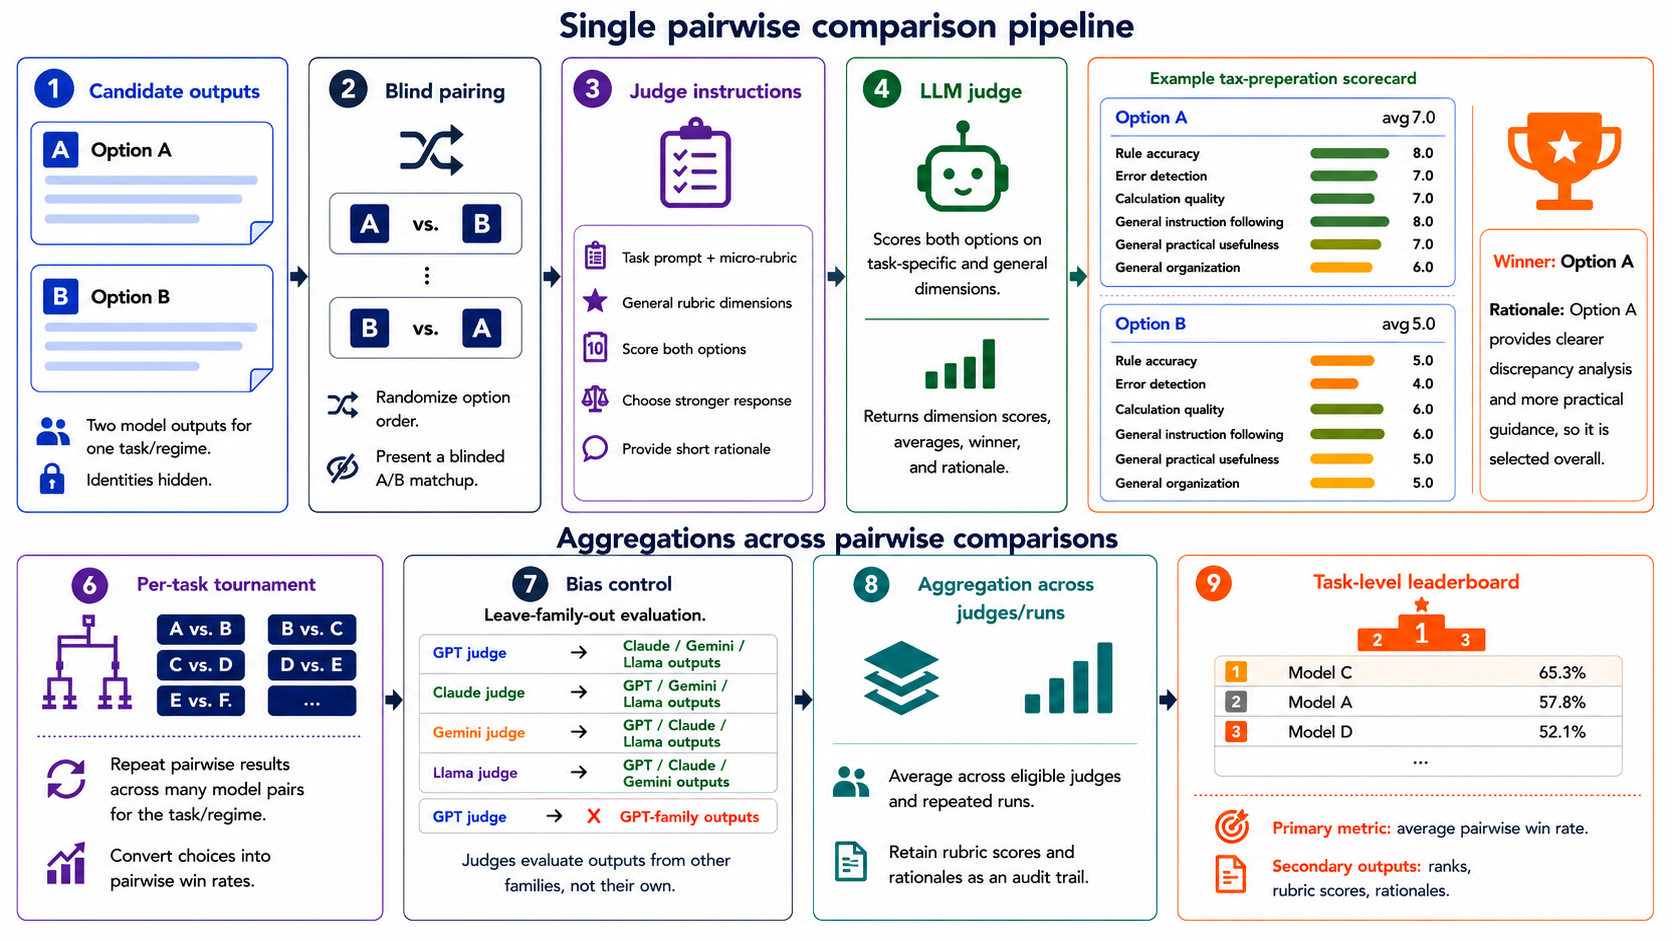
\includegraphics[width=\linewidth]{figures/eval-pipeline.png}
\caption{\textbf{Rubric-guided pairwise evaluation pipeline.} Candidate outputs are anonymized, randomly paired, and evaluated by LLM judges using task-specific and general rubric dimensions. Pairwise choices are converted into win rates, aggregated across eligible judges and repeated runs, and reported alongside rubric scores and rationales as an audit trail.}
\label{fig:eval-pipeline}
\end{figure}

% Following prior work on LLM-as-judge evaluation \citep{zheng2023} and pairwise preference benchmarking \citep{chiang2024}, we evaluate final outputs using blind pairwise comparisons conducted by a panel of LLM judges. Prior research finds that LLM judgments can achieve substantial agreement with human preferences when model identities are concealed and evaluators receive explicit criteria. Figure~\ref{fig:eval-pipeline} summarizes our evaluation pipeline.

Following prior work on LLM-as-judge evaluation and pairwise preference benchmarking \citep{zheng2023,chiang2024}, we evaluate final outputs through blind pairwise comparisons conducted by a panel of four LLM judges. Figure~\ref{fig:eval-pipeline} summarizes the procedure.

%Within each task and each usage mode, we run a complete round-robin over the ten models, scored by a panel of four LLM judges across ten independent runs, with each judge excluded from comparisons involving its own model family (assistant models and judge panel in Appendix~\ref{app:models}). In augmentation, the candidate pool also includes a \emph{plain} baseline—the fixed worker model with no assistance from external models—as a reference point for whether the assistant model helps at all. For each task and regime, candidate outputs are paired against one another, with model identities hidden from the evaluator and option order randomized. The evaluator scores both options explicitly across the task-specific and general rubric dimensions, averages the scores across all dimensions, and then selects the stronger response overall. To increase transparency, we also prompt the evaluator to provide a short rationale supporting their choice. Pairwise comparisons are conducted within a regime; automation and augmentation outputs are never judged against each other directly. Cross-mode comparison is made at the level of ranks, not raw pairwise outcomes. Across non-tied comparisons, judges' final choices agree with the option receiving the higher average rubric score in 99.7\% of cases, indicating that pairwise outcomes are directionally consistent with the underlying dimension-level evaluations rather than arbitrary preferences (Appendix~\ref{app:llm-judge-validity}). 

For each task, usage mode, and independent run, we conduct a complete round-robin tournament among the ten candidate outputs. In augmentation, this candidate set includes the \emph{plain} baseline: the fixed worker operating without an assistance text. This baseline indicates whether receiving assistance improves the worker's output at all. Automation and augmentation
outputs are evaluated in separate tournaments and are never compared directly. 

For every comparison, model identities are concealed and option order is randomized. The judge scores both responses from 1 to 10 on the task-specific and general rubric dimensions, computes an average score for each response, selects the stronger response, and provides a short rationale. We apply \emph{leave-family-out} evaluation: a judge does not evaluate comparisons containing outputs from its own model family. The model and judge panels are reported in the supplementary document.

We treat pairwise comparison and rubric-based scoring as complementary components of our evaluation pipeline. Pairwise judgments provide the primary ranking signal because relative comparisons can recover expert-intended quality orderings more reliably and with lower annotation time than absolute rubric scores in judgment-intensive professional tasks \citep{yang2026judgmentbench}. More broadly, rubric-guided pairwise LLM judgments have been shown to align closely with human preferences \citep{zheng2023}. Pairwise choices alone, however, reveal which response is preferred without fully explaining why. Dimension-level rubric scores provide an inspectable diagnostic record, identifying the specific strengths and weaknesses underlying each comparison and supporting our qualitative analysis. Because rubric-based evaluation is itself sensitive to score calibration, scale use, and score-option ordering \citep{xu2026pointwisepairwise}, we use standardized rubric-derived rankings as a robustness check rather than as a replacement for pairwise comparison. We therefore use pairwise outcomes to construct the primary rankings and standardized rubric scores to interpret those rankings and test their robustness. Together, the two signals make the evaluation more reliable, transparent, and diagnostically useful. Across non-tied comparisons, the selected response receives the higher mean rubric score in 99.7\% of cases. In addition to the consistency between a judge's choice and its own rubric scores, we also measure agreement across judges. We separately assess inter-judge
reliability across all runs. Across 6,265 comparisons evaluated by at least two eligible judges, the judges select the same winner in 71.0\% of cases. Agreement is higher in automation (74.5\%) than in augmentation (67.8\%). The supplementary document reports the full LLM-judge reliability analysis.

\begin{figure}[htbp]
\centering
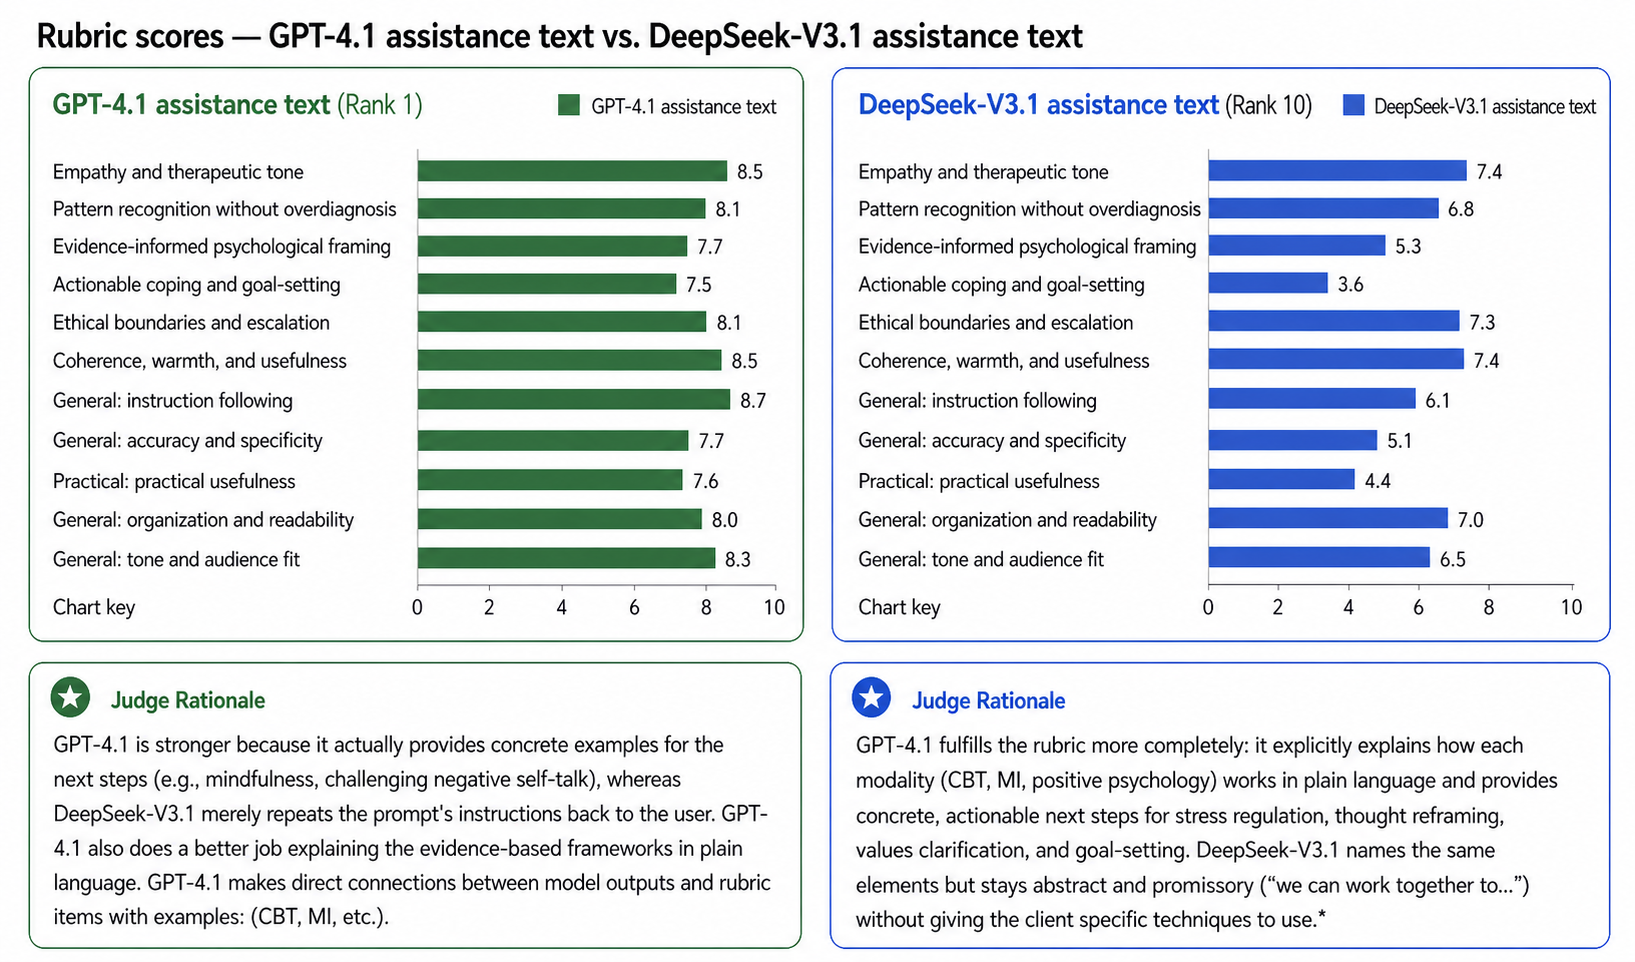
\includegraphics[width=0.87\linewidth]{figures/eval-example.png}
\caption{\textbf{Rubric-guided scoring.} Judge rationales explain the pairwise choice made. The models used in this example are GPT-4.1 and DeepSeek-V3.1 in augmentation mode for the counseling task. The corresponding outputs are in the supplementary document.}
\label{fig:eval-example}
\end{figure}

We aggregate the evaluations in three stages. First, each judge's choices are converted into a pairwise win rate for every model within each task and usage mode.
Second, models are ranked by win rate, and their ranks are averaged across eligible judges and ten independent runs. Third, task-level ranks are combined through a rank-of-ranks aggregation to obtain an overall ordering for each usage mode. We retain all task-level rankings, rubric scores, and rationales for subsequent analysis.

Figure~\ref{fig:eval-example} illustrates the resulting audit trail using two counseling outputs from augmentation mode. It reports the dimension-level
scores and judge rationale for outputs produced with assistance texts from GPT-4.1 and DeepSeek-V3.1. The corresponding assistance texts and final worker
outputs appear in the supplementary document.

% An example is provided in Figure~\ref{fig:eval-example}. It shows the rubric-specific scores for outputs assisted by GPT-4.1 (ranked overall best) and assisted by DeepSeek-V3.1 (ranked overall worst) for the counseling task in the first run. The LLM judge rationale is also included at the bottom of the figure. To see the output for each augmenter, please refer to Appendix~\ref{app:eval-examples}.

% Our ranking pipeline proceeds in four steps. First, for each task and regime, every candidate output is compared pairwise against every other candidate, with model identities hidden and option order randomized. Second, each eligible judge's pairwise choices are converted into a per-model win rate. Third, within each task and regime, models are ordered by average win rate to produce a per-judge ranking, which we average across eligible judges (under leave-one-family-out masking) and across runs. Fourth, we combine these task-level average ranks into a single ordering per regime using a rank-of-ranks aggregation, while retaining the task-level rankings used throughout our analyses.
